\section[System]{System Overview}

\begin{frame}{LG-Loc System Architecture}
    \begin{columns}
        \begin{column}{.6\textwidth}
            \begin{itemize}
                \item Users launch the \textbf{localization application} upon entering a \textbf{building} and obtain their \textbf{location};
                \item Application requests the building's \textbf{landmark graph};
                \item Data used for \textbf{landmark detection} and \textbf{location estimation};
                \item Initial location obtained via:
                    \begin{itemize}
                        \item \textit{WiFi fingerprinting} (if database is \textbf{available});
                        \item \textit{HMM-based algorithm} (if database is \textbf{unavailable}).
                    \end{itemize}
            \end{itemize}
        \end{column}
        \begin{column}{.4\textwidth}
            \begin{figure}[t]
                \centering
                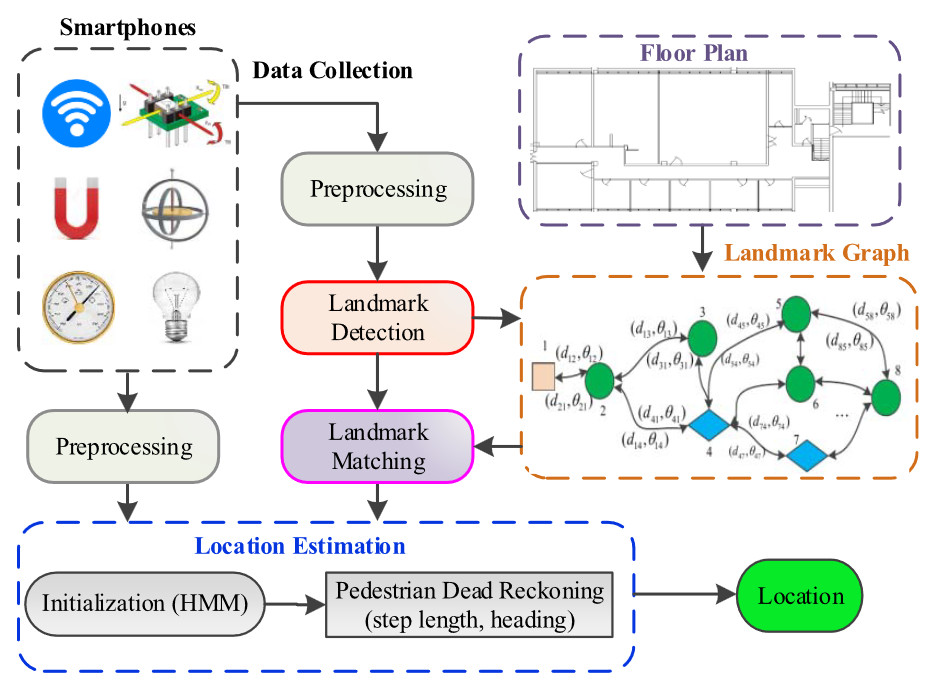
\includegraphics[width=\linewidth]{images/sys.jpg}
                \caption{System architecture of LG-Loc}
                \label{fig:sys}
            \end{figure}
        \end{column}
    \end{columns}
\end{frame}